\documentclass[12pt]{article}
\usepackage[english]{babel}
\usepackage[utf8]{inputenc}
\usepackage{amsmath, amssymb, amsthm}
\usepackage{graphicx}
\usepackage{hyperref}
\usepackage[margin=.75in]{geometry}
\usepackage{xcolor}
\usepackage{tikz}
\usepackage{gensymb}

\setlength{\topmargin}{0pt}
\setlength{\headsep}{0pt}
\textheight = 600pt

\title{Graph Theory \\ Homework 8}
\author{Ben Kallus and Nicholas Adair}
\date{Due Monday, Monday, March 15}

\begin{document}
\maketitle

\noindent{\bf 4.25}

    The following are all of the spanning trees for $G$:
    \begin{center}
        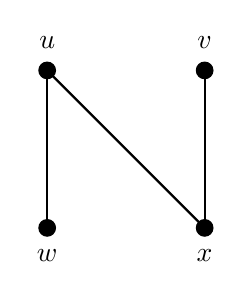
\begin{tikzpicture}
            \draw[fill=black] (0.0, 2.0) circle (3pt);
            \node at (0.0, 2.35) {$u$};
            \draw[fill=black] (0.0, 0.0) circle (3pt);
            \node at (0.0, -0.35) {$w$};
            \draw[fill=black] (2.0, 0.0) circle (3pt);
            \node at (2.0, -0.35) {$x$};
            \draw[fill=black] (2.0, 2.0) circle (3pt);
            \node at (2.0, 2.35) {$v$};

            \draw[thick] (0.0, 2.0) -- (0.0, 0.0); % u-w
            \draw[thick] (0.0, 2.0) -- (2.0, 0.0); % u-x
            \draw[thick] (2.0, 2.0) -- (2.0, 0.0); % v-x
        \end{tikzpicture}
        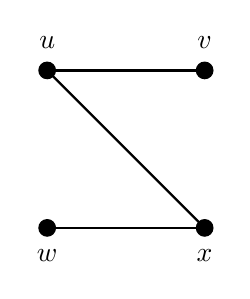
\begin{tikzpicture}
            \draw[fill=black] (0.0, 2.0) circle (3pt);
            \node at (0.0, 2.35) {$u$};
            \draw[fill=black] (0.0, 0.0) circle (3pt);
            \node at (0.0, -0.35) {$w$};
            \draw[fill=black] (2.0, 0.0) circle (3pt);
            \node at (2.0, -0.35) {$x$};
            \draw[fill=black] (2.0, 2.0) circle (3pt);
            \node at (2.0, 2.35) {$v$};

            \draw[thick] (0.0, 2.0) -- (2.0, 0.0); % u-x
            \draw[thick] (0.0, 2.0) -- (2.0, 2.0); % u-v
            \draw[thick] (0.0, 0.0) -- (2.0, 0.0); % w-x
        \end{tikzpicture}
        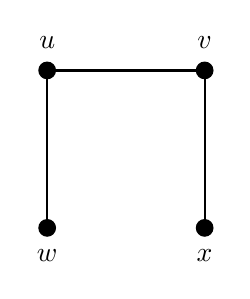
\begin{tikzpicture}
            \draw[fill=black] (0.0, 2.0) circle (3pt);
            \node at (0.0, 2.35) {$u$};
            \draw[fill=black] (0.0, 0.0) circle (3pt);
            \node at (0.0, -0.35) {$w$};
            \draw[fill=black] (2.0, 0.0) circle (3pt);
            \node at (2.0, -0.35) {$x$};
            \draw[fill=black] (2.0, 2.0) circle (3pt);
            \node at (2.0, 2.35) {$v$};

            \draw[thick] (0.0, 2.0) -- (0.0, 0.0); % u-w
            \draw[thick] (0.0, 2.0) -- (2.0, 2.0); % u-v
            \draw[thick] (2.0, 2.0) -- (2.0, 0.0); % v-x
        \end{tikzpicture}
        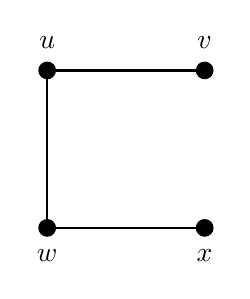
\begin{tikzpicture}
            \draw[fill=black] (0.0, 2.0) circle (3pt);
            \node at (0.0, 2.35) {$u$};
            \draw[fill=black] (0.0, 0.0) circle (3pt);
            \node at (0.0, -0.35) {$w$};
            \draw[fill=black] (2.0, 0.0) circle (3pt);
            \node at (2.0, -0.35) {$x$};
            \draw[fill=black] (2.0, 2.0) circle (3pt);
            \node at (2.0, 2.35) {$v$};

            \draw[thick] (0.0, 2.0) -- (0.0, 0.0); % u-w
            \draw[thick] (0.0, 2.0) -- (2.0, 2.0); % u-v
            \draw[thick] (0.0, 0.0) -- (2.0, 0.0); % w-x
        \end{tikzpicture}
        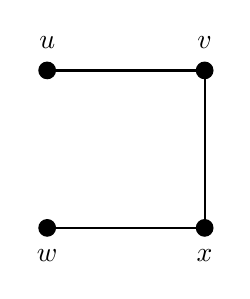
\begin{tikzpicture}
            \draw[fill=black] (0.0, 2.0) circle (3pt);
            \node at (0.0, 2.35) {$u$};
            \draw[fill=black] (0.0, 0.0) circle (3pt);
            \node at (0.0, -0.35) {$w$};
            \draw[fill=black] (2.0, 0.0) circle (3pt);
            \node at (2.0, -0.35) {$x$};
            \draw[fill=black] (2.0, 2.0) circle (3pt);
            \node at (2.0, 2.35) {$v$};

            \draw[thick] (0.0, 2.0) -- (2.0, 2.0); % u-v
            \draw[thick] (0.0, 0.0) -- (2.0, 0.0); % w-x
            \draw[thick] (2.0, 2.0) -- (2.0, 0.0); % v-x
        \end{tikzpicture}
        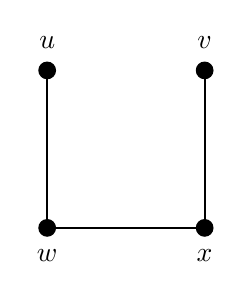
\begin{tikzpicture}
            \draw[fill=black] (0.0, 2.0) circle (3pt);
            \node at (0.0, 2.35) {$u$};
            \draw[fill=black] (0.0, 0.0) circle (3pt);
            \node at (0.0, -0.35) {$w$};
            \draw[fill=black] (2.0, 0.0) circle (3pt);
            \node at (2.0, -0.35) {$x$};
            \draw[fill=black] (2.0, 2.0) circle (3pt);
            \node at (2.0, 2.35) {$v$};

            \draw[thick] (0.0, 2.0) -- (0.0, 0.0); % u-w
            \draw[thick] (0.0, 0.0) -- (2.0, 0.0); % w-x
            \draw[thick] (2.0, 2.0) -- (2.0, 0.0); % v-x
        \end{tikzpicture}

        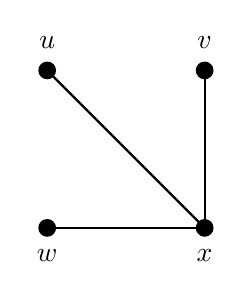
\begin{tikzpicture}
            \draw[fill=black] (0.0, 2.0) circle (3pt);
            \node at (0.0, 2.35) {$u$};
            \draw[fill=black] (0.0, 0.0) circle (3pt);
            \node at (0.0, -0.35) {$w$};
            \draw[fill=black] (2.0, 0.0) circle (3pt);
            \node at (2.0, -0.35) {$x$};
            \draw[fill=black] (2.0, 2.0) circle (3pt);
            \node at (2.0, 2.35) {$v$};

            \draw[thick] (0.0, 2.0) -- (2.0, 0.0); % u-x
            \draw[thick] (0.0, 0.0) -- (2.0, 0.0); % w-x
            \draw[thick] (2.0, 2.0) -- (2.0, 0.0); % v-x
        \end{tikzpicture}
        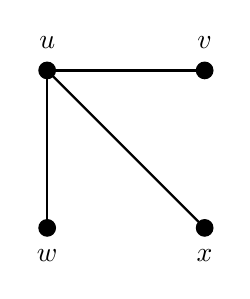
\begin{tikzpicture}
            \draw[fill=black] (0.0, 2.0) circle (3pt);
            \node at (0.0, 2.35) {$u$};
            \draw[fill=black] (0.0, 0.0) circle (3pt);
            \node at (0.0, -0.35) {$w$};
            \draw[fill=black] (2.0, 0.0) circle (3pt);
            \node at (2.0, -0.35) {$x$};
            \draw[fill=black] (2.0, 2.0) circle (3pt);
            \node at (2.0, 2.35) {$v$};

            \draw[thick] (0.0, 2.0) -- (0.0, 0.0); % u-w
            \draw[thick] (0.0, 2.0) -- (2.0, 0.0); % u-x
            \draw[thick] (0.0, 2.0) -- (2.0, 2.0); % u-v
        \end{tikzpicture}
    \end{center}

    The first row of spanning trees are all isomorphic, since they are all $P_3$.
    The second row of spanning trees are isomorphic, since the graph on the left can be obtained from the graph on the right through a $180\degree$ rotation.

    We can be certain that these are all possible spanning trees for $G$.
    Since $G$ is of order 4, a spanning tree for $G$ must have 3 edges.
    Since $G$ is of size 5, each spanning tree of $G$ can be obtained from $G$ by removing 2 edges from $G$.
    Thus, there are at most ${5 \choose 2} = 10$ spanning trees for $G$.
    Since removing $uv,uw$ or $xv,xw$ would disconnect the graph, there are at most 8 spanning trees for $G$.
    Thus, we have found all spanning trees for $G$.

    \newpage
    The following are all of the spanning trees for $H$:
    \begin{center}
        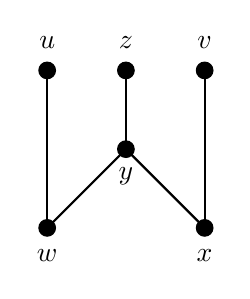
\begin{tikzpicture}
            \draw[fill=black] (0.0, 0.0) circle (3pt);
            \node at (0.0, -0.35) {$w$};
            \draw[fill=black] (1.0, 1.0) circle (3pt);
            \node at (1.0, .65) {$y$};
            \draw[fill=black] (2.0, 0.0) circle (3pt);
            \node at (2.0, -0.35) {$x$};
            \draw[fill=black] (2.0, 2.0) circle (3pt);
            \node at (2.0, 2.35) {$v$};
            \draw[fill=black] (0.0, 2.0) circle (3pt);
            \node at (0.0, 2.35) {$u$};
            \draw[fill=black] (1.0, 2.0) circle (3pt);
            \node at (1.0, 2.35) {$z$};

            \draw[thick] (0.0, 2.0) -- (0.0, 0.0); % u-w
            \draw[thick] (0.0, 0.0) -- (1.0, 1.0); % w-y
            \draw[thick] (2.0, 0.0) -- (1.0, 1.0); % y-x
            \draw[thick] (2.0, 2.0) -- (2.0, 0.0); % v-x
            \draw[thick] (1.0, 1.0) -- (1.0, 2.0); % y-z
        \end{tikzpicture}
        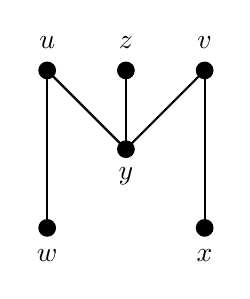
\begin{tikzpicture}
            \draw[fill=black] (0.0, 0.0) circle (3pt);
            \node at (0.0, -0.35) {$w$};
            \draw[fill=black] (1.0, 1.0) circle (3pt);
            \node at (1.0, .65) {$y$};
            \draw[fill=black] (2.0, 0.0) circle (3pt);
            \node at (2.0, -0.35) {$x$};
            \draw[fill=black] (2.0, 2.0) circle (3pt);
            \node at (2.0, 2.35) {$v$};
            \draw[fill=black] (0.0, 2.0) circle (3pt);
            \node at (0.0, 2.35) {$u$};
            \draw[fill=black] (1.0, 2.0) circle (3pt);
            \node at (1.0, 2.35) {$z$};

            \draw[thick] (0.0, 2.0) -- (0.0, 0.0); % u-w
            \draw[thick] (1.0, 1.0) -- (0.0, 2.0); % u-y
            \draw[thick] (1.0, 1.0) -- (2.0, 2.0); % y-v
            \draw[thick] (2.0, 2.0) -- (2.0, 0.0); % v-x
            \draw[thick] (1.0, 1.0) -- (1.0, 2.0); % y-z
        \end{tikzpicture}
        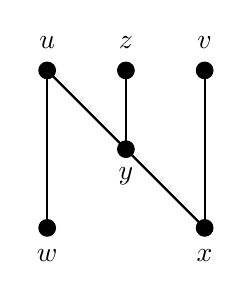
\begin{tikzpicture}
            \draw[fill=black] (0.0, 0.0) circle (3pt);
            \node at (0.0, -0.35) {$w$};
            \draw[fill=black] (1.0, 1.0) circle (3pt);
            \node at (1.0, .65) {$y$};
            \draw[fill=black] (2.0, 0.0) circle (3pt);
            \node at (2.0, -0.35) {$x$};
            \draw[fill=black] (2.0, 2.0) circle (3pt);
            \node at (2.0, 2.35) {$v$};
            \draw[fill=black] (0.0, 2.0) circle (3pt);
            \node at (0.0, 2.35) {$u$};
            \draw[fill=black] (1.0, 2.0) circle (3pt);
            \node at (1.0, 2.35) {$z$};

            \draw[thick] (0.0, 2.0) -- (0.0, 0.0); % u-w
            \draw[thick] (1.0, 1.0) -- (0.0, 2.0); % u-y
            \draw[thick] (2.0, 0.0) -- (1.0, 1.0); % y-x
            \draw[thick] (2.0, 2.0) -- (2.0, 0.0); % v-x
            \draw[thick] (1.0, 1.0) -- (1.0, 2.0); % y-z
        \end{tikzpicture}
        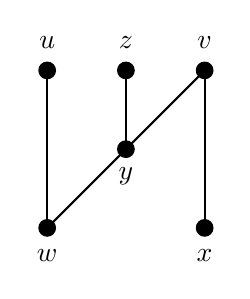
\begin{tikzpicture}
            \draw[fill=black] (0.0, 0.0) circle (3pt);
            \node at (0.0, -0.35) {$w$};
            \draw[fill=black] (1.0, 1.0) circle (3pt);
            \node at (1.0, .65) {$y$};
            \draw[fill=black] (2.0, 0.0) circle (3pt);
            \node at (2.0, -0.35) {$x$};
            \draw[fill=black] (2.0, 2.0) circle (3pt);
            \node at (2.0, 2.35) {$v$};
            \draw[fill=black] (0.0, 2.0) circle (3pt);
            \node at (0.0, 2.35) {$u$};
            \draw[fill=black] (1.0, 2.0) circle (3pt);
            \node at (1.0, 2.35) {$z$};

            \draw[thick] (0.0, 2.0) -- (0.0, 0.0); % u-w
            \draw[thick] (0.0, 0.0) -- (1.0, 1.0); % w-y
            \draw[thick] (1.0, 1.0) -- (2.0, 2.0); % y-v
            \draw[thick] (2.0, 2.0) -- (2.0, 0.0); % v-x
            \draw[thick] (1.0, 1.0) -- (1.0, 2.0); % y-z
        \end{tikzpicture}

        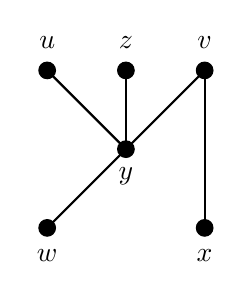
\begin{tikzpicture}
            \draw[fill=black] (0.0, 0.0) circle (3pt);
            \node at (0.0, -0.35) {$w$};
            \draw[fill=black] (1.0, 1.0) circle (3pt);
            \node at (1.0, .65) {$y$};
            \draw[fill=black] (2.0, 0.0) circle (3pt);
            \node at (2.0, -0.35) {$x$};
            \draw[fill=black] (2.0, 2.0) circle (3pt);
            \node at (2.0, 2.35) {$v$};
            \draw[fill=black] (0.0, 2.0) circle (3pt);
            \node at (0.0, 2.35) {$u$};
            \draw[fill=black] (1.0, 2.0) circle (3pt);
            \node at (1.0, 2.35) {$z$};

            \draw[thick] (0.0, 0.0) -- (1.0, 1.0); % w-y
            \draw[thick] (1.0, 1.0) -- (0.0, 2.0); % u-y
            \draw[thick] (1.0, 1.0) -- (2.0, 2.0); % y-v
            \draw[thick] (2.0, 2.0) -- (2.0, 0.0); % v-x
            \draw[thick] (1.0, 1.0) -- (1.0, 2.0); % y-z
        \end{tikzpicture}
        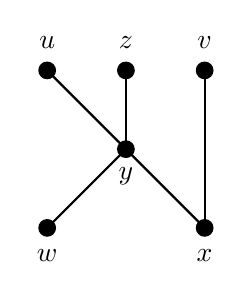
\begin{tikzpicture}
            \draw[fill=black] (0.0, 0.0) circle (3pt);
            \node at (0.0, -0.35) {$w$};
            \draw[fill=black] (1.0, 1.0) circle (3pt);
            \node at (1.0, .65) {$y$};
            \draw[fill=black] (2.0, 0.0) circle (3pt);
            \node at (2.0, -0.35) {$x$};
            \draw[fill=black] (2.0, 2.0) circle (3pt);
            \node at (2.0, 2.35) {$v$};
            \draw[fill=black] (0.0, 2.0) circle (3pt);
            \node at (0.0, 2.35) {$u$};
            \draw[fill=black] (1.0, 2.0) circle (3pt);
            \node at (1.0, 2.35) {$z$};

            \draw[thick] (0.0, 0.0) -- (1.0, 1.0); % w-y
            \draw[thick] (1.0, 1.0) -- (0.0, 2.0); % u-y
            \draw[thick] (2.0, 0.0) -- (1.0, 1.0); % y-x
            \draw[thick] (2.0, 2.0) -- (2.0, 0.0); % v-x
            \draw[thick] (1.0, 1.0) -- (1.0, 2.0); % y-z
        \end{tikzpicture}
        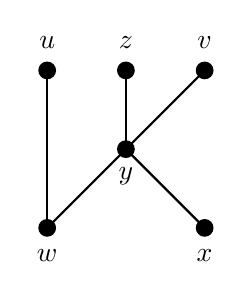
\begin{tikzpicture}
            \draw[fill=black] (0.0, 0.0) circle (3pt);
            \node at (0.0, -0.35) {$w$};
            \draw[fill=black] (1.0, 1.0) circle (3pt);
            \node at (1.0, .65) {$y$};
            \draw[fill=black] (2.0, 0.0) circle (3pt);
            \node at (2.0, -0.35) {$x$};
            \draw[fill=black] (2.0, 2.0) circle (3pt);
            \node at (2.0, 2.35) {$v$};
            \draw[fill=black] (0.0, 2.0) circle (3pt);
            \node at (0.0, 2.35) {$u$};
            \draw[fill=black] (1.0, 2.0) circle (3pt);
            \node at (1.0, 2.35) {$z$};

            \draw[thick] (0.0, 2.0) -- (0.0, 0.0); % u-w
            \draw[thick] (0.0, 0.0) -- (1.0, 1.0); % w-y
            \draw[thick] (2.0, 0.0) -- (1.0, 1.0); % y-x
            \draw[thick] (1.0, 1.0) -- (2.0, 2.0); % y-v
            \draw[thick] (1.0, 1.0) -- (1.0, 2.0); % y-z
        \end{tikzpicture}
        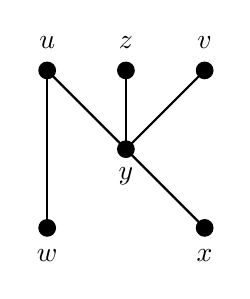
\begin{tikzpicture}
            \draw[fill=black] (0.0, 0.0) circle (3pt);
            \node at (0.0, -0.35) {$w$};
            \draw[fill=black] (1.0, 1.0) circle (3pt);
            \node at (1.0, .65) {$y$};
            \draw[fill=black] (2.0, 0.0) circle (3pt);
            \node at (2.0, -0.35) {$x$};
            \draw[fill=black] (2.0, 2.0) circle (3pt);
            \node at (2.0, 2.35) {$v$};
            \draw[fill=black] (0.0, 2.0) circle (3pt);
            \node at (0.0, 2.35) {$u$};
            \draw[fill=black] (1.0, 2.0) circle (3pt);
            \node at (1.0, 2.35) {$z$};

            \draw[thick] (0.0, 2.0) -- (0.0, 0.0); % u-w
            \draw[thick] (1.0, 1.0) -- (0.0, 2.0); % u-y
            \draw[thick] (2.0, 0.0) -- (1.0, 1.0); % y-x
            \draw[thick] (1.0, 1.0) -- (2.0, 2.0); % y-v
            \draw[thick] (1.0, 1.0) -- (1.0, 2.0); % y-z
        \end{tikzpicture}

        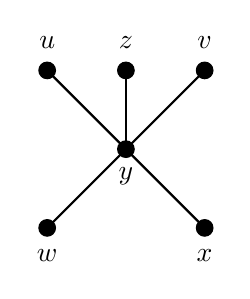
\begin{tikzpicture}
            \draw[fill=black] (0.0, 0.0) circle (3pt);
            \node at (0.0, -0.35) {$w$};
            \draw[fill=black] (1.0, 1.0) circle (3pt);
            \node at (1.0, .65) {$y$};
            \draw[fill=black] (2.0, 0.0) circle (3pt);
            \node at (2.0, -0.35) {$x$};
            \draw[fill=black] (2.0, 2.0) circle (3pt);
            \node at (2.0, 2.35) {$v$};
            \draw[fill=black] (0.0, 2.0) circle (3pt);
            \node at (0.0, 2.35) {$u$};
            \draw[fill=black] (1.0, 2.0) circle (3pt);
            \node at (1.0, 2.35) {$z$};

            \draw[thick] (0.0, 0.0) -- (1.0, 1.0); % w-y
            \draw[thick] (1.0, 1.0) -- (0.0, 2.0); % u-y
            \draw[thick] (2.0, 0.0) -- (1.0, 1.0); % y-x
            \draw[thick] (1.0, 1.0) -- (2.0, 2.0); % y-v
            \draw[thick] (1.0, 1.0) -- (1.0, 2.0); % y-z
        \end{tikzpicture}
    \end{center}

    The first row of spanning trees are all isomorphic, since they can % ANNOYING TO WRITE.
    REMEMBER TO COME BACK AND FINISH THIS LATER. ANNOYING TO WRITE IT ALL OUT.

    We can be certain that these are all possible spanning trees for $H$. Since $H$ is of order 6, a spanning tree for $H$ must have 5 edges.
    Since $H$ is of size 7, each spanning tree of $H$ can be obtained from $H$ by removing 2 edges from $H$.
    Since $yz$ is a bridge, it must be present in any spanning tree of $H$.
    Since removing any two of $\{uy, wy, uw\}$ would disconnect the graph, at least two of the edges in that set must be present in any spanning tree of $H$.
    Similarly, at least two of $\{vy, xy, vx\}$ must be present in any spanning tree of $H$.
    Thus, each spanning tree of $H$ can be expressed as $H - e_1 - e_2$ for some $e_1 \in \{uy, wy, uw\}$, and some $e_2 \in \{vy, xy, vx\}$.
    Thus, there are ${3 \choose 1} \cdot {3 \choose 1} = 9$ spanning trees of $H$.

\newpage\noindent{\bf 4.26} Proposition: An edge $e$ of a connected graph $G$ is a bridge if and only if $e$ belongs to every spanning tree of $G$.
\begin{proof}
    Let $G$ be a connected graph.
    Let $e \in E(G)$.

    Suppose that $e$ is a bridge.
    Then, $G-e$ is disconnected.
    Thus, every connected spanning subgraph of $G$ contains $e$.
    Thus, every spanning tree of $G$ contains $e$.

    Now, suppose that every spanning tree of $G$ contains $e$.
    Assume, toward a contradiction, that $e$ is not a bridge.
    Then, $G-e$ is connected.
    Let $T$ be a spanning tree of $G-e$.
    Then, $e \notin E(T)$.
    Since $G-e$ is connected, $T$ is also a spanning tree of $G$.
    Thus, we have contradicted our assumption, so $e$ must be a bridge in $G$.

    Thus, $e$ is a bridge in $G$ if and only if $e$ belongs to every spanning tree of $G$.
\end{proof}

\newpage\noindent{\bf 4.27}

Kruskal's Algorithm:
\begin{center}
    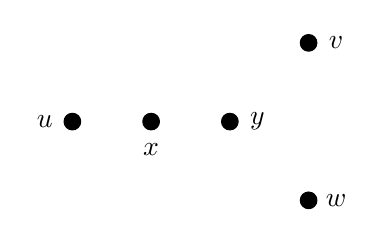
\begin{tikzpicture}
        \draw[fill=black] (0.0, 0.0) circle (3pt);
        \node at (-0.35, 0.0) {$u$};
        \draw[fill=black] (1.0, 0.0) circle (3pt);
        \node at (1.0, -.35) {$x$};
        \draw[fill=black] (2.0, 0.0) circle (3pt);
        \node at (2.35, 0.0) {$y$};
        \draw[fill=black] (3.0, 1.0) circle (3pt);
        \node at (3.35, 1.0) {$v$};
        \draw[fill=black] (3.0, -1.0) circle (3pt);
        \node at (3.35, -1.0) {$w$};
    \end{tikzpicture}

    $\downarrow$

    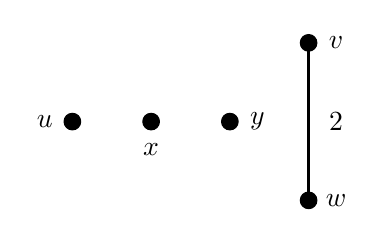
\begin{tikzpicture}
        \draw[fill=black] (0.0, 0.0) circle (3pt);
        \node at (-0.35, 0.0) {$u$};
        \draw[fill=black] (1.0, 0.0) circle (3pt);
        \node at (1.0, -.35) {$x$};
        \draw[fill=black] (2.0, 0.0) circle (3pt);
        \node at (2.35, 0.0) {$y$};
        \draw[fill=black] (3.0, 1.0) circle (3pt);
        \node at (3.35, 1.0) {$v$};
        \draw[fill=black] (3.0, -1.0) circle (3pt);
        \node at (3.35, -1.0) {$w$};

        \draw[thick] (3.0, -1.0) -- (3.0, 1.0);
        \node at (3.35, 0) {2};
    \end{tikzpicture}

    $\downarrow$

    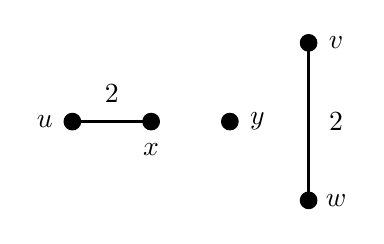
\begin{tikzpicture}
        \draw[fill=black] (0.0, 0.0) circle (3pt);
        \node at (-0.35, 0.0) {$u$};
        \draw[fill=black] (1.0, 0.0) circle (3pt);
        \node at (1.0, -.35) {$x$};
        \draw[fill=black] (2.0, 0.0) circle (3pt);
        \node at (2.35, 0.0) {$y$};
        \draw[fill=black] (3.0, 1.0) circle (3pt);
        \node at (3.35, 1.0) {$v$};
        \draw[fill=black] (3.0, -1.0) circle (3pt);
        \node at (3.35, -1.0) {$w$};

        \draw[thick] (3.0, -1.0) -- (3.0, 1.0);
        \node at (3.35, 0) {2};
        \draw[thick] (0,0) -- (1,0);
        \node at (.5,.35) {2};
    \end{tikzpicture}

    $\downarrow$

    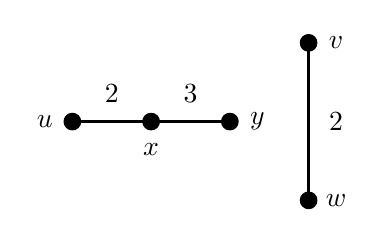
\begin{tikzpicture}
        \draw[fill=black] (0.0, 0.0) circle (3pt);
        \node at (-0.35, 0.0) {$u$};
        \draw[fill=black] (1.0, 0.0) circle (3pt);
        \node at (1.0, -.35) {$x$};
        \draw[fill=black] (2.0, 0.0) circle (3pt);
        \node at (2.35, 0.0) {$y$};
        \draw[fill=black] (3.0, 1.0) circle (3pt);
        \node at (3.35, 1.0) {$v$};
        \draw[fill=black] (3.0, -1.0) circle (3pt);
        \node at (3.35, -1.0) {$w$};

        \draw[thick] (3.0, -1.0) -- (3.0, 1.0);
        \node at (3.35, 0) {2};
        \draw[thick] (0,0) -- (1,0);
        \node at (.5,.35) {2};
        \draw[thick] (1.0,0) -- (2,0);
        \node at (1.5,.35) {3};
    \end{tikzpicture}

    $\downarrow$

    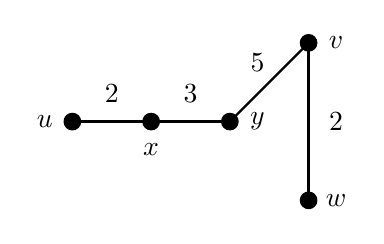
\begin{tikzpicture}
        \draw[fill=black] (0.0, 0.0) circle (3pt);
        \node at (-0.35, 0.0) {$u$};
        \draw[fill=black] (1.0, 0.0) circle (3pt);
        \node at (1.0, -.35) {$x$};
        \draw[fill=black] (2.0, 0.0) circle (3pt);
        \node at (2.35, 0.0) {$y$};
        \draw[fill=black] (3.0, 1.0) circle (3pt);
        \node at (3.35, 1.0) {$v$};
        \draw[fill=black] (3.0, -1.0) circle (3pt);
        \node at (3.35, -1.0) {$w$};

        \draw[thick] (3.0, -1.0) -- (3.0, 1.0);
        \node at (3.35, 0) {2};
        \draw[thick] (0,0) -- (1,0);
        \node at (.5,.35) {2};
        \draw[thick] (1.0,0) -- (2,0);
        \node at (1.5,.35) {3};
        \draw[thick] (2,0) -- (3,1);
        \node at (2.35, .75) {5};
    \end{tikzpicture}
\end{center}

\newpage
Prim's Algorithm:
\begin{center}
    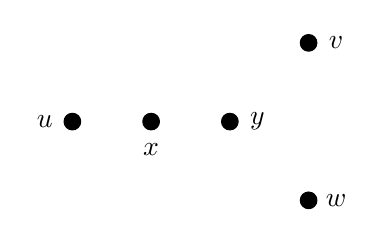
\begin{tikzpicture}
        \draw[fill=black] (0.0, 0.0) circle (3pt);
        \node at (-0.35, 0.0) {$u$};
        \draw[fill=black] (1.0, 0.0) circle (3pt);
        \node at (1.0, -.35) {$x$};
        \draw[fill=black] (2.0, 0.0) circle (3pt);
        \node at (2.35, 0.0) {$y$};
        \draw[fill=black] (3.0, 1.0) circle (3pt);
        \node at (3.35, 1.0) {$v$};
        \draw[fill=black] (3.0, -1.0) circle (3pt);
        \node at (3.35, -1.0) {$w$};

        % \draw[thick] (3.0, -1.0) -- (3.0, 1.0);
        % \node at (3.35, 0) {2};
        % \draw[thick] (0,0) -- (1,0);
        % \node at (.5,.35) {2};
        % \draw[thick] (1.0,0) -- (2,0);
        % \node at (1.5,.35) {3};
        % \draw[thick] (2,0) -- (3,1);
        % \node at (2.35, .75) {5};
    \end{tikzpicture}

    $\downarrow$

    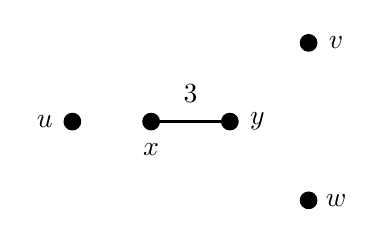
\begin{tikzpicture}
        \draw[fill=black] (0.0, 0.0) circle (3pt);
        \node at (-0.35, 0.0) {$u$};
        \draw[fill=black] (1.0, 0.0) circle (3pt);
        \node at (1.0, -.35) {$x$};
        \draw[fill=black] (2.0, 0.0) circle (3pt);
        \node at (2.35, 0.0) {$y$};
        \draw[fill=black] (3.0, 1.0) circle (3pt);
        \node at (3.35, 1.0) {$v$};
        \draw[fill=black] (3.0, -1.0) circle (3pt);
        \node at (3.35, -1.0) {$w$};

        % \draw[thick] (3.0, -1.0) -- (3.0, 1.0);
        % \node at (3.35, 0) {2};
        % \draw[thick] (0,0) -- (1,0);
        % \node at (.5,.35) {2};
        \draw[thick] (1.0,0) -- (2,0);
        \node at (1.5,.35) {3};
        % \draw[thick] (2,0) -- (3,1);
        % \node at (2.35, .75) {5};
    \end{tikzpicture}

    $\downarrow$

    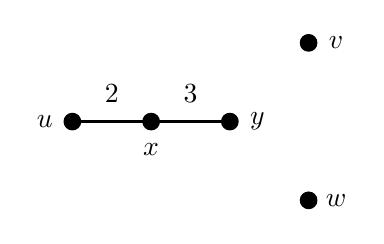
\begin{tikzpicture}
        \draw[fill=black] (0.0, 0.0) circle (3pt);
        \node at (-0.35, 0.0) {$u$};
        \draw[fill=black] (1.0, 0.0) circle (3pt);
        \node at (1.0, -.35) {$x$};
        \draw[fill=black] (2.0, 0.0) circle (3pt);
        \node at (2.35, 0.0) {$y$};
        \draw[fill=black] (3.0, 1.0) circle (3pt);
        \node at (3.35, 1.0) {$v$};
        \draw[fill=black] (3.0, -1.0) circle (3pt);
        \node at (3.35, -1.0) {$w$};

        % \draw[thick] (3.0, -1.0) -- (3.0, 1.0);
        % \node at (3.35, 0) {2};
        \draw[thick] (0,0) -- (1,0);
        \node at (.5,.35) {2};
        \draw[thick] (1.0,0) -- (2,0);
        \node at (1.5,.35) {3};
        % \draw[thick] (2,0) -- (3,1);
        % \node at (2.35, .75) {5};
    \end{tikzpicture}

    $\downarrow$

    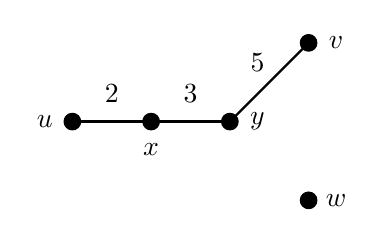
\begin{tikzpicture}
        \draw[fill=black] (0.0, 0.0) circle (3pt);
        \node at (-0.35, 0.0) {$u$};
        \draw[fill=black] (1.0, 0.0) circle (3pt);
        \node at (1.0, -.35) {$x$};
        \draw[fill=black] (2.0, 0.0) circle (3pt);
        \node at (2.35, 0.0) {$y$};
        \draw[fill=black] (3.0, 1.0) circle (3pt);
        \node at (3.35, 1.0) {$v$};
        \draw[fill=black] (3.0, -1.0) circle (3pt);
        \node at (3.35, -1.0) {$w$};

        % \draw[thick] (3.0, -1.0) -- (3.0, 1.0);
        % \node at (3.35, 0) {2};
        \draw[thick] (0,0) -- (1,0);
        \node at (.5,.35) {2};
        \draw[thick] (1.0,0) -- (2,0);
        \node at (1.5,.35) {3};
        \draw[thick] (2,0) -- (3,1);
        \node at (2.35, .75) {5};
    \end{tikzpicture}

    $\downarrow$

    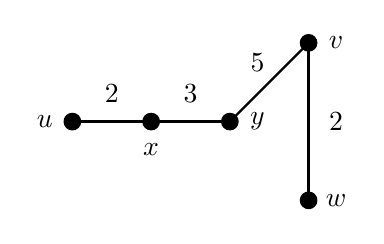
\begin{tikzpicture}
        \draw[fill=black] (0.0, 0.0) circle (3pt);
        \node at (-0.35, 0.0) {$u$};
        \draw[fill=black] (1.0, 0.0) circle (3pt);
        \node at (1.0, -.35) {$x$};
        \draw[fill=black] (2.0, 0.0) circle (3pt);
        \node at (2.35, 0.0) {$y$};
        \draw[fill=black] (3.0, 1.0) circle (3pt);
        \node at (3.35, 1.0) {$v$};
        \draw[fill=black] (3.0, -1.0) circle (3pt);
        \node at (3.35, -1.0) {$w$};

        \draw[thick] (3.0, -1.0) -- (3.0, 1.0);
        \node at (3.35, 0) {2};
        \draw[thick] (0,0) -- (1,0);
        \node at (.5,.35) {2};
        \draw[thick] (1.0,0) -- (2,0);
        \node at (1.5,.35) {3};
        \draw[thick] (2,0) -- (3,1);
        \node at (2.35, .75) {5};
    \end{tikzpicture}
\end{center}

\newpage\noindent{\bf ALSO}

\noindent{\bf 1.}

$S-e+f_1$:
\begin{center}
    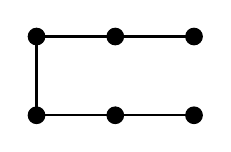
\begin{tikzpicture}
        \draw[fill=black] (0.0, 0.0) circle (3pt);
        \draw[fill=black] (1.0, 0.0) circle (3pt);
        \draw[fill=black] (2.0, 0.0) circle (3pt);
        \draw[fill=black] (0.0, 1.0) circle (3pt);
        \draw[fill=black] (1.0, 1.0) circle (3pt);
        \draw[fill=black] (2.0, 1.0) circle (3pt);

        \draw[thick] (0,0) -- (1,0);
        \draw[thick] (1,0) -- (2,0);
        \draw[thick] (2,1) -- (1,1);
        \draw[thick] (1,1) -- (0,1);
        \draw[thick] (0,1) -- (0,0); % f_1
    \end{tikzpicture}
\end{center}

$T+e-f_1:$
\begin{center}
    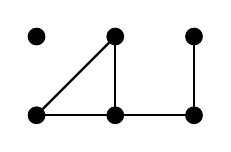
\begin{tikzpicture}
        \draw[fill=black] (0.0, 0.0) circle (3pt);
        \draw[fill=black] (1.0, 0.0) circle (3pt);
        \draw[fill=black] (2.0, 0.0) circle (3pt);
        \draw[fill=black] (0.0, 1.0) circle (3pt);
        \draw[fill=black] (1.0, 1.0) circle (3pt);
        \draw[fill=black] (2.0, 1.0) circle (3pt);

        \draw[thick] (0,0) -- (1,0);
        \draw[thick] (1,0) -- (2,0);
        \draw[thick] (2,0) -- (2,1); % f_3
        \draw[thick] (0,0) -- (1,1); % f_2
        \draw[thick] (1,1) -- (1,0); % e
    \end{tikzpicture}
\end{center}

$S-e+f_2:$
\begin{center}
    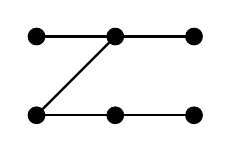
\begin{tikzpicture}
        \draw[fill=black] (0.0, 0.0) circle (3pt);
        \draw[fill=black] (1.0, 0.0) circle (3pt);
        \draw[fill=black] (2.0, 0.0) circle (3pt);
        \draw[fill=black] (0.0, 1.0) circle (3pt);
        \draw[fill=black] (1.0, 1.0) circle (3pt);
        \draw[fill=black] (2.0, 1.0) circle (3pt);

        \draw[thick] (0,0) -- (1,0);
        \draw[thick] (1,0) -- (2,0);
        \draw[thick] (2,1) -- (1,1);
        \draw[thick] (1,1) -- (0,1);
        \draw[thick] (0,0) -- (1,1); % f_2
    \end{tikzpicture}
\end{center}

$T+e-f_2:$
\begin{center}
    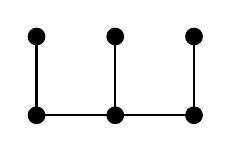
\begin{tikzpicture}
        \draw[fill=black] (0.0, 0.0) circle (3pt);
        \draw[fill=black] (1.0, 0.0) circle (3pt);
        \draw[fill=black] (2.0, 0.0) circle (3pt);
        \draw[fill=black] (0.0, 1.0) circle (3pt);
        \draw[fill=black] (1.0, 1.0) circle (3pt);
        \draw[fill=black] (2.0, 1.0) circle (3pt);

        \draw[thick] (0,0) -- (1,0);
        \draw[thick] (1,0) -- (2,0);
        \draw[thick] (2,0) -- (2,1); % f_3
        \draw[thick] (0,1) -- (0,0); % f_1
        \draw[thick] (1,1) -- (1,0); % e
    \end{tikzpicture}
\end{center}

$S-e+f_3:$
\begin{center}
    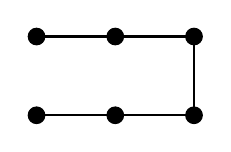
\begin{tikzpicture}
        \draw[fill=black] (0.0, 0.0) circle (3pt);
        \draw[fill=black] (1.0, 0.0) circle (3pt);
        \draw[fill=black] (2.0, 0.0) circle (3pt);
        \draw[fill=black] (0.0, 1.0) circle (3pt);
        \draw[fill=black] (1.0, 1.0) circle (3pt);
        \draw[fill=black] (2.0, 1.0) circle (3pt);

        \draw[thick] (0,0) -- (1,0);
        \draw[thick] (1,0) -- (2,0);
        \draw[thick] (2,1) -- (1,1);
        \draw[thick] (1,1) -- (0,1);
        \draw[thick] (2,0) -- (2,1); % f_3
    \end{tikzpicture}
\end{center}

$T+e-f_3:$
\begin{center}
    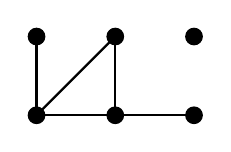
\begin{tikzpicture}
        \draw[fill=black] (0.0, 0.0) circle (3pt);
        \draw[fill=black] (1.0, 0.0) circle (3pt);
        \draw[fill=black] (2.0, 0.0) circle (3pt);
        \draw[fill=black] (0.0, 1.0) circle (3pt);
        \draw[fill=black] (1.0, 1.0) circle (3pt);
        \draw[fill=black] (2.0, 1.0) circle (3pt);

        \draw[thick] (0,0) -- (1,0);
        \draw[thick] (1,0) -- (2,0);
        \draw[thick] (0,1) -- (0,0); % f_1
        \draw[thick] (0,0) -- (1,1); % f_2
        \draw[thick] (1,1) -- (1,0); % e
    \end{tikzpicture}
\end{center}

\newpage\noindent{\bf 2.}

Lemma: If $T$ is a tree, then $T+uv$ contains at most 1 cycle for all $u,v \in V(T)$.
\begin{proof}
    Let $T$ be a tree.
    Let $u,v \in V(T)$.
    Consider the following two cases:

    {\bf Case 1.} $uv \in E(T)$. \\
    Then, $T + uv = T$, so $T + uv$ is a tree and thus contains no cycles.

    {\bf Case 2.} $uv \notin E(T)$. \\
    Suppose that $T + uv$ contains the distinct cycles $A$ and $B$.
    Then, since $T$ is a tree, $uv$ is in both $A$ and $B$.
    Therefore, it is safe to assume that $A$ and $B$ are both of the form $(v, \hdots, u, v)$.\footnote{If they are not, simply rotate them until they are.}
    Let $P_A$ be the $v-u$ path obtained by removing the final entry from $A$.
    Let $P_B$ be the $v-u$ path obtained by removing the final entry from $B$.
    Note that $P_A \neq P_B$, since $A \neq B$.
    Let $P$ be the concatenation $P_A$ with the reverse of $P_B$.
    Since $P$ is a circuit, and $P$ does not contain $uv$, it must be that $T$ contains a cycle.
    Thus, $T$ is not a tree, so a contradiction has been demonstrated.
    Therefore, $T+uv$ contains less than 2 cycles.
\end{proof}

Proposition: If $S$ and $T$ are spanning trees of a connected graph $G$, then for every edge $e \in E(S) \setminus E(T)$, there is an edge $f \in E(T) \setminus E(S)$ such that $S-e+f$ and $T+e-f$ are both spanning trees of $G$.
\begin{proof}
    Let $G$ be a connected graph.
    Let $S$ and $T$ be spanning trees of $G$.
    Let $e=uv \in E(S) \setminus E(T)$.

    Then, $S - e$ consists of two components, one containing $u$ and the other containing $v$.
    By Theorem 4.2, there is a unique $u-v$ path $P = (u, p_1, \hdots, v)$ in $T$.
    Thus, there exists an edge $f$ along $P$ that connects the components of $S - e$.
    Thus, $f$ is a bridge in $S - e + f$.
    Thus, every edge in $S-e+f$ is a bridge, so $S-e+f$ is a tree.
    Since $S-e+f$ is a tree with the same size and vertex set as $S$, $S-e+f$ is therefore a spanning tree of $G$.

    Note that $P$ has length at least 2, since $e \notin E(T)$.
    Thus, $C = (u, p_1, \hdots, v, u)$ is a cycle in $T+e$.
    Then, by the lemma above, $C$ is the only cycle in $T+e$.
    Note that since $e \in E(S)$, $f \neq e$.
    Since removing $f$ from $T+e$ would remove the cycle $C$, $T+e-f$ thus has no cycles.
    Since $f$ lies on a cycle of $T+e$, $f$ is not a bridge in $T+e$, so $T+e-f$ is connected.
    Thus, $T+e-f$ is a tree.
    Since $T+e-f$ is a tree with the same size and vertex set as $T$, $T+e-f$ is therefore a spanning tree of $G$.
\end{proof}

\newpage\noindent{\bf 4.30} Proposition: A connected weighted graph $G$ has a unique spanning tree $T$ if and only if the weight of each edge $e$ of $G$ that is not in $T$ exceeds the weight of every other edge on the cycle in $T+e$.
\begin{proof}
    Let $G$ be a connected. weighted graph.

    Suppose that $G$ has a unique spanning tree, $T$.
    Let $e \in E(G) \setminus E(T)$.
    By the lemma in the previous proof, $T+e$ has at most one cycle.
    Since $T$ is a spanning tree of $G$, $T+e$ has $n$ edges, and is therefore not a tree.
    Thus, $T+e$ contains exactly one cycle.
    Suppose $w(e) = w(f)$ for some edge $f \neq e$ along the cycle in $T+e$.
    Then, since $f$ lies along a cycle in $T+e$, it is not a bridge in $T+e$.
    Thus, $T+e-f$ is connected, and has no cycles.
    Thus, $T+e-f$ is a tree with $n-1$ edges and the same vertex set as $G$.
    Thus, $T+e-f$ is a minimum spanning tree for $G$.
    Since $e \neq f$, $T+e-f \neq T$.
    Thus, $G$ does not have a unique minimum spanning tree, so it must be that $w(e) \neq w(f)$ for all $f \neq e$ along the cycle in $T+e$.

    DO THE REST OF THIS.
\end{proof}

\newpage\noindent{\bf 5.2}

    {\bf (a)} For each integer $k \geq 2$, $K_{k,1}$ is a connected graph containing a vertex $v$ such that $G-v$ has $k$ components.
    This vertex is the only element of the order 1 partite set.

    {\bf (b)} $K_2 \cup K_1$ is an example of such a graph.
    To see this, assign $u$ and $v$ to be the vertices in the $K_2$ component of the graph.

\newpage\noindent{\bf 5.4}

    

\end{document}